% !TeX root = ../main.tex
% Appendix A -- supplementary information for a research chapter.  Figures and tables are
% numbered A.1, A.2, ...  The [H] placement keeps supplementary figures in order.
\chapter{SUPPLEMENTARY INFORMATION FOR CHAPTER 2}
\label{app:supplementary}

\begin{chapternote}
This appendix reproduces the Supplementary Information for Chapter~\ref{ch:manuscript}. Supplementary Figure~\textit{N} of the published article corresponds to Figure~A.\textit{N} here.
\end{chapternote}

\section{Supplementary Figures}

\begin{figure}[H]
\centering
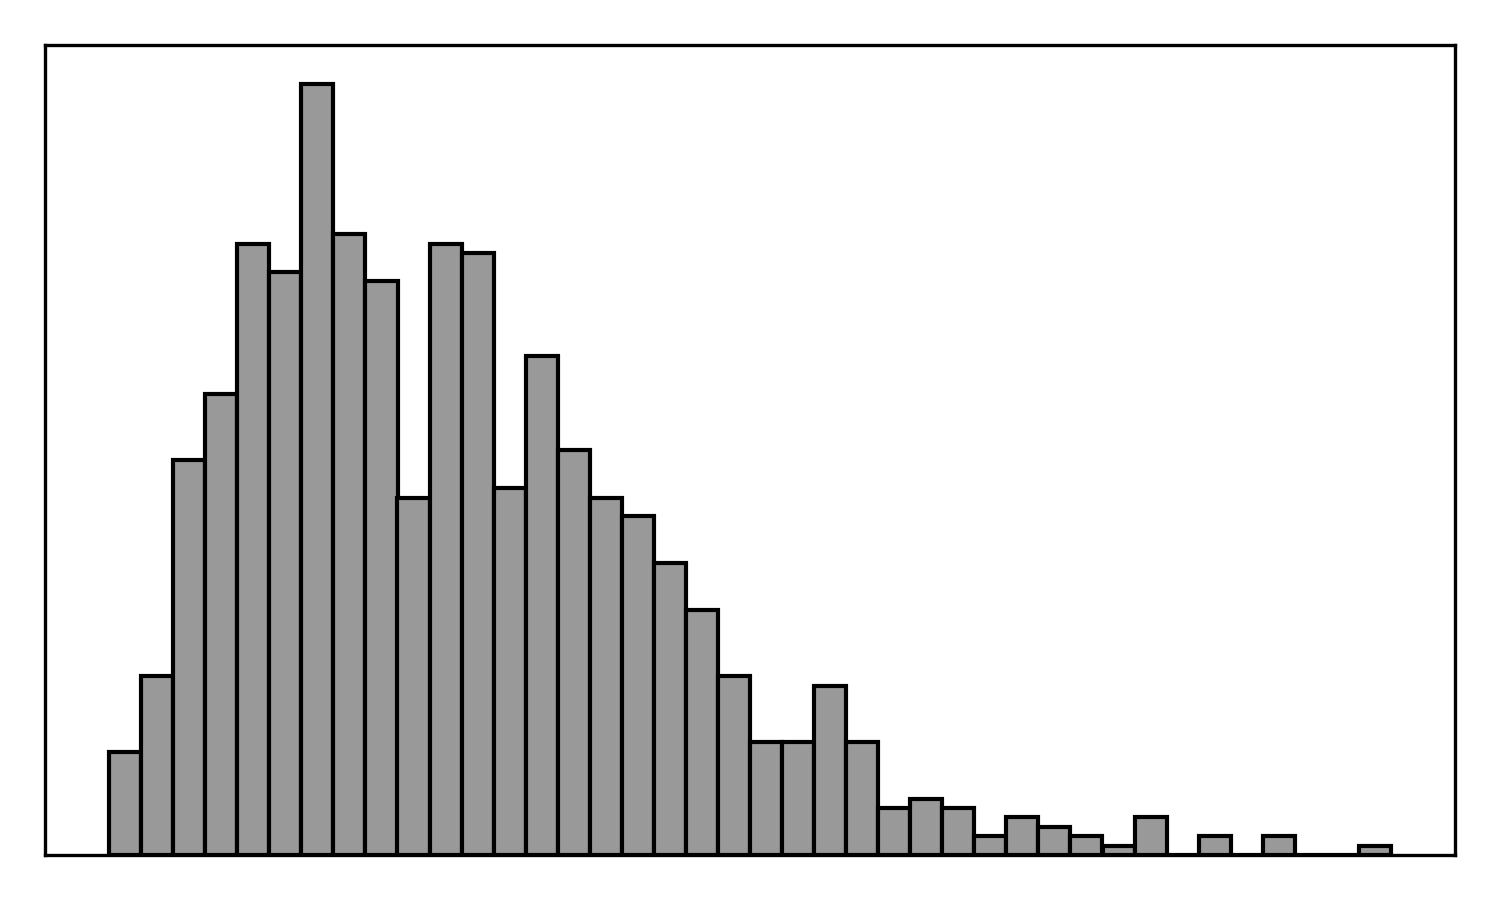
\includegraphics[width=0.8\textwidth,keepaspectratio]{figures/example-supplementary.png}
\caption[Example of a supplementary figure]{\textbf{Example of a supplementary figure.} Replace this legend with the supplementary figure legend.}
\label{fig:appA:example}
\end{figure}

\section{Supplementary Tables}

Wide tables can be set on a landscape page. The page number stays at the bottom of the page in portrait orientation, as the Graduate School requires.

\begin{landscape}
{\singlespacing
\tablesmall\setlength{\tabcolsep}{4pt}
\begin{longtable}{@{}p{1.3in}p{1.3in}p{1.3in}p{1.3in}p{1.3in}p{1.3in}@{}}
\caption[Example of a wide table on a landscape page]{\textbf{Example of a wide table on a landscape page.} Long tables continue across pages, and the header row is repeated.}
\label{tab:appA:wide}\\
\toprule
\textbf{Column 1} & \textbf{Column 2} & \textbf{Column 3} & \textbf{Column 4} & \textbf{Column 5} & \textbf{Column 6}\\
\midrule
\endfirsthead
\multicolumn{6}{@{}l}{\textit{Table \thetable\ (continued)}}\\
\toprule
\textbf{Column 1} & \textbf{Column 2} & \textbf{Column 3} & \textbf{Column 4} & \textbf{Column 5} & \textbf{Column 6}\\
\midrule
\endhead
\bottomrule
\endlastfoot
Row 1 & Value & Value & Value & Value & Value\\
Row 2 & Value & Value & Value & Value & Value\\
Row 3 & Value & Value & Value & Value & Value\\
\end{longtable}}
\end{landscape}
